\باب{برق گیر اور امالہ گیر}

\حصہ{برق گیر}
متوازی چادر \اصطلاح{برق گیر}\فرہنگ{برق گیر}\حاشیہب{capacitor}\فرہنگ{capacitor} جسے شکل \حوالہ{شکل_امالہ_متوازی_چادر}-الف میں دکھایا گیا ہے کے بارے میں آپ نے چھوٹی جماعتوں میں پڑھا ہو گا۔خالی خلاء میں دو عدد یکساں، سیدھے متوازی موصل چادر جن کے مابین فاصلہ \عددی{d} ہو اور  ایک چادر کا رقبہ \عددی{S} ہو کی \اصطلاح{برقی گنجائش}\فرہنگ{برقی گنجائش}\فرہنگ{گنجائش!برقی}\حاشیہب{capacitance}\فرہنگ{capacitance} \عددی{C} درج ذیل مساوات دیتی ہے
\begin{align}\label{مساوات_امالہ_تعریف_مساوات}
C=\frac{\epsilon_0 S}{d}
\end{align}
جہاں \عددی{\epsilon_0} خالی خلاء کا \اصطلاح{برقی مستقل}\فرہنگ{برقی مستقل}\حاشیہب{permitivity, electric constant}\فرہنگ{permitivity}\فرہنگ{electric constant} ہے جس کی قیمت \عددی{\SI{8.85e-12}{\farad\per\meter}} ہے۔برقی گنجائش کو کولمب فی وولٹ \عددی{\si{\coulomb\per\volt}} یا فیراڈ \عددی{\si{\farad}} میں ناپا جاتا ہے۔فیراڈ\حاشیہد{فیراڈ کی اکائی انگلستان کے مشہور ماہر طبیعیات مائکل فیراڈے کے نام سے منسوب ہے۔} کی اکائی انتہائی بڑی مقدار ہے  لہٰذا برقی گنجائش کو عموماً مائکرو فیراڈ \عددی{\si{\micro\farad}} اور نینو فیراڈ \عددی{\nano\farad} میں ناپا جاتا ہے۔
%=================
\ابتدا{مثال}
متوازی چادر برق گیر میں چادروں کے مابین فاصلہ \عددی{\SI{0.1}{\milli\meter}} ہے جبکہ اس کی برقی گنجائش \عددی{\SI{0.1}{\micro\farad}} ہے۔ایک چادر کا رقبہ دریافت کریں۔

حل:مساوات \حوالہ{مساوات_امالہ_تعریف_مساوات} استعمال کرتے ہوئے
\begin{align*}
S=\frac{C d}{\epsilon_0}=\frac{0.1\times 10^{-6} \times 0.1\times 10^{-3}}{8.854\times 10^{-12}}=\SI{1.129}{\meter\squared}
\end{align*}
حاصل ہوتا ہے۔
\انتہا{مثال}
%===================

\begin{figure}
\centering
\begin{subfigure}{0.5\textwidth}
\centering
\begin{tikzpicture}
\draw(\x/2+\x/8,0)--++(0,-\y/2) to [short,-o]++(-\x,0);
\draw[fill=white,opacity=1](0,-\dy)--++(\x,0)--++(\x/4,\y/2)--++(-\x,0)--++(-\x/4,-\y/2);
\draw[fill=white,opacity=1](0,0)--++(\x,0)--++(\x/4,\y/2)--++(-\x,0)--++(-\x/4,-\y/2);
\draw(\x/2+\x/8,\y/4)--++(0,\y/2) to [short,-o]++(-\x,0);
\draw(\x/4,\y/8)node{$S$};
\draw(\x+\x/4,\y/2)++(\dx,0)--++(2*\dx,0)coordinate(kup);
\draw(\x+\x/4,\y/2-\dy)++(\dx,0)--++(2*\dx,0)coordinate(klow);
\draw[stealth-] (kup)++(-\dx,0)--++(0,\dy)node[above]{$d$};
\draw[stealth-](klow)++(-\dx,0)--++(0,-\dy);
\end{tikzpicture}
\caption*{(الف)}
\end{subfigure}%
\begin{subfigure}{0.5\textwidth}
\centering
\begin{tikzpicture}
\draw(\dx,\dy) to [short,-o]++(\x/2,0) to [short]++(\x,0) to [capacitor,l={$C$}]++(0,\y) to [short,i<_={${i(t)=\frac{\dif q(t)}{\dif t}}$},-o]++(-\x,0) to [short]++(-\x/2,0);  
\draw[fill=white,opacity=1] plot [smooth cycle] coordinates {(0,0) (\x/4,0) (\x/4,\y+2*\dy) (0,\y+2*\dy)};
\draw(\x/2+\dx,\y/2+\dy) node{$\begin{aligned} &+ \\ &v(t) \\ &- \end{aligned}$};
\draw(\x/2+\x+\x/4+\dx,\y/2+\dy) node[right]{$\begin{aligned} &+ \\ & q(t) \\ &- \end{aligned}$};
\end{tikzpicture}
\caption*{(ب)}
\end{subfigure}%
\caption{متوازی چادر برق گیر۔}
\label{شکل_امالہ_متوازی_چادر}
\end{figure}

شکل \حوالہ{شکل_امالہ_متوازی_چادر}-ب میں برقی گیر کو \عددی{v(t)} منبع دباو کے ساتھ جوڑا گیا ہے  جس کی وجہ سے برگ گیر کے ایک چادر پر مثبت برقی بار \عددی{+q(t)} اور دوسرے چادر پر منفی برقی بار \عددی{-q(t)} رو نما ہوتا ہے جبکہ دونوں چادروں کے مابین دباو \عددی{v(t)} پایا جاتا ہے۔برق گیر کے چادروں پر بار اور ان کے مابین دباو خطی تعلق
\begin{align}\label{مساوات_امالہ_بار_دباو_تعلق}
q(t)=C v(t)
\end{align}
رکھتے ہیں جہاں خطی تعلق کے مستقل کو \عددی{C} سے ظاہر اور  \اصطلاح{برقی گنجائش}\فرہنگ{برقی گنجائش}\فرہنگ{گنجائش!برقی}\حاشیہب{capacitance}\فرہنگ{capacitance} کہتے ہیں۔ برقی گنجائش کے نام کو چھوٹا کرتے ہوئے عموماً \اصطلاح{گنجائش} کہا جاتا ہے۔وقت کے ساتھ بدلتی بار کو برقی رو کہا جاتا ہے۔یوں برق گیر کے چادروں پر بار کی تبدیلی رو کو جنم دیتی ہے جسے
\begin{align}
i=\frac{\dif q}{\dif t}
\end{align}
لکھا جا سکتا ہے جسے شکل \حوالہ{شکل_امالہ_متوازی_چادر}-ب میں دکھایا گیا ہے۔برق گیر کے مثبت برقی سر پر مثبت رو داخل ہوتی ہے۔یوں مزاحمت کی طرح  برق گیر پر بھی دباو اور رو انفعالی رائج سمت کے تحت ہیں۔ مساوات \حوالہ{مساوات_امالہ_بار_دباو_تعلق} کو استعمال کرتے ہوئے 
\begin{align}
i=\frac{\dif (C v)}{\dif t}
\end{align}
لکھا جا سکتا ہے۔مستقل برقی گنجائش کی صورت میں اسے
\begin{align}\label{مساوات_امالہ_بار_دباو_تعلق_ب}
i=C\frac{\dif v}{\dif t}
\end{align}
لکھا جا سکتا ہے۔مساوات \حوالہ{مساوات_امالہ_بار_دباو_تعلق_ب} کو
\begin{align*}
\dif v = \frac{1}{C} i \dif t
\end{align*}
لکھ کر تکمل لینے سے
\begin{align}\label{مساوات_امالہ_بار_دباو_تعلق_پ}
v(t)=\frac{1}{C} \int_{-\infty}^{t} i \dif t
\end{align}
حاصل ہوتا ہے جہاں \عددی{t = -\infty} پر برق گیر کا دباو \عددی{v(-\infty) = 0} لیا گیا ہے۔مندرجہ بالا مساوات میں \عددی{v(t)} لکھ کر وقت کو \اصطلاح{آزاد متغیر}\فرہنگ{آزاد متغیر}\حاشیہب{independent variable}\فرہنگ{independent variable} اور دباو کو \اصطلاح{تابع متغیر}\فرہنگ{تابع متغیر}\حاشیہب{dependent variable}\فرہنگ{dependent variable} کے طور پر لکھا گیا ہے۔اس مساوات کو دو ٹکڑوں میں درج ذیل لکھا جا سکتا ہے
\begin{gather}
\begin{aligned}\label{مساوات_امالہ_ابتدائی_دباو_الف}
v(t)&=\frac{1}{C} \int_{-\infty}^{t_0} i \dif t+\frac{1}{C} \int_{t_0}^{t} i \dif t\\
&=v(t_0)+\frac{1}{C} \int_{t_0}^{t} i \dif t
\end{aligned}
\end{gather}
جہاں وقت \عددی{t=-\infty} تا \عددی{t=t_0} کے دوران برق گیر پر جمع ہونے والے بار کی وجہ سے  برق گیر پر وقت \عددی{t=t_0} پر دباو \عددی{v(t_0)} پایا جاتا ہے۔ 

برق گیر میں ذخیرہ توانائی \عددی{w_C(t)} کو طاقت کے تکمل سے حاصل کیا جا سکتا ہے۔برق گیر کو منتقل طاقت \عددی{p(t)} کو
\begin{align}\label{مساوات_امالہ_طاقت_برق_گیر}
p(t)=v(t)i(t)=v(t) C \frac{\dif v(t)}{\dif t}
\end{align}
لکھا جا سکتا ہے۔چونکہ \عددی{p=\tfrac{\dif w}{\dif t}} کے برابر ہے  لہٰذا برق گیر میں ذخیرہ توانائی کو
\begin{align*}
w_C(t)&=\int_{-\infty}^{t} C v(t) \frac{\dif v(t)}{\dif t} \dif t\\
&=C\int_{v(-\infty)}^{v(t)} v(t) \dif v(t)\\
&=\left. C \frac{v^2(t)}{2} \right|_{v(-\infty)}^{v(t)}
\end{align*}
یعنی
\begin{align}\label{مسوات_امالہ_توانائی_برق_گیر_الف}
w_C(t)=\frac{C v^2(t)}{2}
\end{align}
لکھا جا سکتا ہے جہاں \عددی{v(-\infty) =0} لیا گیا ہے۔مساوات \حوالہ{مساوات_امالہ_بار_دباو_تعلق} کی مدد سے اس مساوات کو درج ذیل لکھا جا سکتا ہے۔
\begin{align}\label{مسوات_امالہ_توانائی_برق_گیر_ب}
w_C(t)=\frac{q^2(t)}{2C}
\end{align}
مساوات \حوالہ{مسوات_امالہ_توانائی_برق_گیر_الف} اور مساوات \حوالہ{مسوات_امالہ_توانائی_برق_گیر_ب} برقی گیر میں ذخیرہ \اصطلاح{مخفی توانائی}\فرہنگ{مخفی توانائی}\فرہنگ{توانائی!مخفی}\حاشیہب{potential energy}\فرہنگ{potential energy} دیتے ہیں۔یہ وہی توانائی ہے جو برق گیر میں بار بھرتے ہوئے خرچ کی جاتی ہے۔

مساوات \حوالہ{مساوات_امالہ_بار_دباو_تعلق_ب} کے تحت برقی گیر پر دباو کے تبدیلی کی شرح اور رو کا راست تناسب تعلق ہے۔چونکہ یک سمتی دباو تبدیل نہیں ہوتی لہٰذا برق گیر پر یک سمتی دباو کی صورت میں اس میں کوئی رو نہیں گزرے گی۔یوں یک سمتی دباو کی نقطہ نظر سے برق گیر کھلا دور ہے لہٰذا ادوار کے یک سمتی حل کے دوران تمام برق گیروں کو کھلے دور تصور کیا جاتا ہے۔

مساوات \حوالہ{مساوات_امالہ_طاقت_برق_گیر} کے تحت برق گیر کو منتقل طاقت، دباو کی شرح تبدیلی  کے راست تناسب ہے۔یوں برق گیر کا دباو فوراً تبدیل کرنے کے لئے لامحدود طاقت درکار ہو گی۔کائنات میں لامحدود طاقت کا منبع نہیں پایا جاتا لہٰذا برق گیر کا دباو فوراً کسی صورت تبدیل نہیں کیا جا سکتا۔اسی حقیقت کو مساوات \حوالہ{مساوات_امالہ_بار_دباو_تعلق_ب} سے بھی سمجھا جا سکتا ہے جس کے تحت دباو فوراً تبدیل کرنے کے لئے لا محدود رو درکار ہو گی۔چونکہ لا محدود رو کہیں نہیں پائی جاتی لہٰذا ایسا ممکن نہیں ہے۔یہ ایک اہم نتیجہ ہے جس کے تحت دور میں سوئچ کو چالو سے غیر چالو (یا غیر چالو سے چالو) کرنے کے فوراً بعد دور میں موجود  برق گیر کے دباو کی قیمت وہی ہو گی جو سوئچ چالو (یا غیر چالو) کرنے سے پہلے تھی۔اس حقیقت کو اگلے باب میں استعمال کیا جائے گا۔

مساوات \حوالہ{مساوات_امالہ_بار_دباو_تعلق} برق گیر کی عمومی مساوات ہے۔کسی بھی دو موصل جن کے درمیان دباو \عددی{v} اور جن میں مثبت موصل پر \عددی{+q} اور منفی موصل پر \عددی{-q} بار پایا جاتا ہو کی گنجائش مساوات \حوالہ{مساوات_امالہ_بار_دباو_تعلق} دیتی ہے۔یوں دور کے مختلف موصل حصوں مثلاً مزاحمت، باقی تار، برق گیر وغیرہ کے مابین \اصطلاح{غیر مطلوب}\فرہنگ{غیر مطلوب}\حاشیہب{stray}\فرہنگ{stray} برقی گنجائش پائی جائے گی۔بعض ادوار میں غیر مطلوب برقی گنجائش کو کم سے کم رکھنا ضروری ہوتا ہے جبکہ یک سمتی ادوار میں ان کے کردار کو رد کیا جاتا ہے
%==============
\ابتدا{مثال}
برق گیر کی دباو \عددی{\SI{20}{\volt}} سے \عددی{\SI{20.1}{\volt}} کرنے کی خاطر منبع رو استعمال کیا جاتا ہے۔برق گیر کی گنجائش \عددی{\SI{1}{\micro\farad}} ہے۔تبدیلی کا دورانیہ ایک سیکنڈ، ایک نینو سیکنڈ، ایک فیمٹو سیکنڈ اور صفر سیکنڈ تصور کرتے ہوئے درکار رو کی قیمت حاصل کریں۔دباو کے تبدیلی کے دوران رو کی قیمت مستقل تصور کریں۔

حل:دورانیہ ایک سیکنڈ تصور کرتے ہوئے مساوات   \حوالہ{مساوات_امالہ_بار_دباو_تعلق_ب} کے تحت
\begin{align*}
i=10^{-6} \times \left(\frac{20.1-20}{1}\right)=\SI{0.1}{\micro\ampere}
\end{align*}
درکار ہو گی۔اسی طرح بالترتیب بقایا دورانیوں کے لئے درج ذیل رو حاصل ہوتی ہیں۔
\begin{align*}
i&=10^{-6} \times \left(\frac{20.1-20}{10^{-9}}\right)=\SI{100}{\ampere}\\
i&=10^{-6} \times \left(\frac{20.1-20}{10^{-15}}\right)=\SI{e8}{\ampere}\\
i&=10^{-6} \times \left(\frac{20.1-20}{0}\right)=\infty\, \si{\ampere}
\end{align*}

\انتہا{مثال}
%=======================
\ابتدا{مثال}

دو  قریبی موصل تاروں پر \عددی{\SI{300}{\nano\coulomb}} بار ذخیرہ کرنے سے ان کے مابین \عددی{\SI{15}{\volt}} دباو پیدا ہوتا ہے۔ان جوڑی موصل کی برقی گنجائش دریافت کریں۔

حل:مساوات \حوالہ{مساوات_امالہ_بار_دباو_تعلق} کے تحت
\begin{align*}
C=\frac{q}{v}=\frac{300 \times 10^{-9}}{15}=\SI{20}{\nano\farad}
\end{align*}
ہو گا۔ 
\انتہا{مثال}
%======================
\ابتدا{مثال}
شکل میں \عددی{\SI{2}{\micro\farad}} برق گیر پر دباو دکھایا گیا ہے۔برق گیر کی رو دریافت کریں۔

\begin{figure}
\centering
\begin{subfigure}{1\textwidth}
\centering
\begin{tikzpicture}
\draw[gray](0,-2)--(0,3)node[left]{$v(t)$};
\draw[gray](0,0)--++(6.5,0)node[right]{$t(\si{\milli\second})$};
\draw(-0.5,0)--(0,0)--++(1,2)--++(1.5,0)--++(2,-3)--++(2,0);
\draw(1,0)--++(0,-0.1)node[below]{$10$};
\draw(2.5,0)--++(0,-0.1)node[below]{$25$};
\draw(4.5,0)--++(0,-0.1)node[below]{$45$};
\draw(0,2)--++(-0.1,0)node[left]{$\SI{50}{\volt}$};
\draw(0,-1)--++(-0.1,0)node[left]{$\SI{-25}{\volt}$};
\end{tikzpicture}
\caption*{(الف)}
\end{subfigure}
\begin{subfigure}{1\textwidth}
\centering
\begin{tikzpicture}
\draw[gray](0,-1)--(0,1.5)node[left]{$i(t)$};
\draw[gray](0,0)--++(6.5,0)node[right]{$t(\si{\milli\second})$};
\draw(-0.5,0)--(0,0)--++(0,1)--++(1,0)--++(0,-1)--++(1.5,0)--++(0,-0.7)--++(2,0)--++(0,0.7)--++(2,0);
\draw(1,0)node[below]{$10$};
\draw(2.5,0)node[above]{$25$};
\draw(4.5,0)node[above]{$45$};
\draw(0,1)--++(-0.1,0)node[left]{$\SI{10}{\milli\ampere}$};
\draw(0,-0.7)--++(-0.1,0)node[left]{$\SI{-7}{\milli\ampere}$};
\end{tikzpicture}
\caption*{(ب)}
\end{subfigure}
\end{figure}

حل:دورانیہ \عددی{\SI{0}{\second}} تا \عددی{\SI{10}{\milli\second}} میں دباو مسلسل مستقل شرح
\begin{align*}
\frac{\Delta v}{\Delta t}=\frac{\SI{50}{\volt}-\SI{0}{\volt}}{\SI{10}{\milli\second}-\SI{0}{\second}}=\SI{5000}{\volt\per\second}
\end{align*}
 سے بڑھتا ہے لہٰذا اس دوران دباو بالمقابل وقت کی مساوات 
\begin{align*}
v(t)=5000 t \quad \quad (0 \le t \le \SI{10}{\milli\second})
\end{align*}
لکھی جا سکتی ہے۔وقت \عددی{\SI{10}{\milli\second}} تا \عددی{\SI{25}{\milli\second}} دباو بغیر تبیل ہوئے مستقل \عددی{\SI{50}{\volt}} پر برقرار رہتا ہے لہٰذا اس دوران دباو کی مساوات درج ذیل ہے۔
\begin{align*}
v(t)=50 \quad \quad (\SI{10}{\milli\second} \le t \le \SI{25}{\milli\second})
\end{align*}
اس کے بعد \عددی{\SI{25}{\milli\second}} تا \عددی{\SI{45}{\milli\second}} کے دوران دباو مستقل شرح
\begin{align*}
\frac{\Delta v}{\Delta t}=\frac{\SI{-25}{\volt}-\SI{50}{\volt}}{\SI{45}{\milli\second}-\SI{25}{\milli\second}}=\SI{-3500}{\volt \per \second}
\end{align*}
سے گھٹتا ہے لہٰذا اس دوران دباو کی مساوات
\begin{align*}
v(t)=-3500 t +75 \quad \quad (\SI{25}{\milli\second} \le t \le \SI{45}{\milli\second})
\end{align*}
ہو گی۔اس کے بعد دباو برقرار \عددی{\SI{-25}{\volt}} پر رہتا ہے لہٰذا اس کی مساوات درج ذیل ہو گی۔
\begin{align*}
v(t)=-25 \quad \quad (\SI{45}{\milli\second} \le t)
\end{align*}
مساوات \حوالہ{مساوات_امالہ_بار_دباو_تعلق_ب} استعمال کرتے ہوئے ان دورانیوں میں رو حاصل کرتے ہیں۔
\begin{align*}
i&=2\times 10^{-6} \times 5000=\SI{10}{\milli\ampere} \quad \quad \quad \quad  (0 \le t \le \SI{10}{\milli\second})\\
i&=2\times 10^{-6} \times 0=\SI{0}{\milli\ampere} \quad \quad \quad \quad \quad   (\SI{10}{\milli\second} \le t \le \SI{25}{\milli\second})\\
i&=2\times 10^{-6} \times (-3500)=\SI{-7}{\milli\ampere} \quad \quad   \quad  (\SI{25}{\milli\second} \le t \le \SI{45}{\milli\second})\\
i&=2\times 10^{-6} \times 0=\SI{0}{\milli\ampere} \quad \quad \quad \quad   \quad(\SI{45}{\milli\second} \le t)
\end{align*}
رو بالمقابل وقت کو شکل-ب میں دکھایا گیا ہے۔
\انتہا{مثال}
%=====================
\ابتدا{مثال}
گزشتہ مثال میں لمحہ \عددی{t=\SI{10}{\milli\second}}، \عددی{t=\SI{20}{\milli\second}} اور \عددی{t=\SI{50}{\milli\second}} پر برق گیر میں ذخیرہ مخفی تونائی دریافت کریں۔

حل:مساوات \حوالہ{مسوات_امالہ_توانائی_برق_گیر_الف} کے تحت جوابات درج ذیل ہیں۔
\begin{align*}
w_C(\SI{10}{\milli\second})&=\frac{2\times 10^{-6}\times 50^2}{2}=\SI{2.5}{\milli\joule}\\
w_C(\SI{20}{\milli\second})&=\frac{2\times 10^{-6}\times 50^2}{2}=\SI{2.5}{\milli\joule}\\
w_C(\SI{50}{\milli\second})&=\frac{2\times 10^{-6}\times (-25)^2}{2}=\SI{0.625}{\milli\joule}
\end{align*}
\انتہا{مثال}
%====================
\ابتدا{مشق}
برق گیر پر ذخیرہ بار کی قیمت \عددی{\SI{5}{\nano\coulomb}} ہے جبکہ اس پر دباو \عددی{\SI{100}{\volt}} ہیں۔برقی گنجائش دریافت کریں۔

جواب:\عددی{\SI{5}{\pico\farad}}
\انتہا{مشق}
%====================
\ابتدا{مثال}
ابتدائی طور پر بے بار \عددی{\SI{22}{\micro\farad}} کے برق گیر کی رو کو شکل \حوالہ{شکل_امالہ_مثال_تبدیل_ہوتی_رو_الف} میں دکھایا گیا ہے۔برق گیر کے دباو، طاقت اور ذخیرہ توانائی کے مساوات حاصل کرتے ہوئے  خط کھینچیں۔

\begin{figure}
\centering
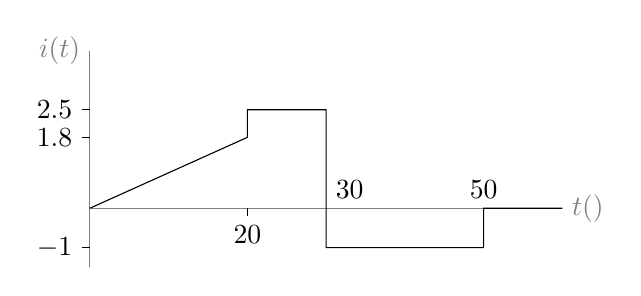
\begin{tikzpicture}
\draw[gray](0,-0.75)--(0,2)node[left]{$i(t)$};
\draw[gray](0,0)--++(6,0)node[right]{$t(\si{\milli\second})$};
\draw(0,0)--++(2,0.9)--++(0,0.35)--++(1,0)--++(0,-1.75)--++(2,0)--++(0,0.5)--++(1,0);
\draw(0,0.9)--++(-0.1,0)node[left]{$\SI{1.8}{\milli\ampere}$};
\draw(0,1.25)--++(-0.1,0)node[left]{$\SI{2.5}{\milli\ampere}$};
\draw(0,-0.5)--++(-0.1,0)node[left]{$\SI{-1}{\milli\ampere}$};
\draw(2,0)--++(0,-0.1)node[below]{$20$};
\draw(3,0)node[above right]{$30$};
\draw(5,0)node[above]{$50$};
\end{tikzpicture}
\caption{(الف)}
\label{شکل_امالہ_مثال_تبدیل_ہوتی_رو_الف}
\end{figure} 

حل:دورانیہ \عددی{t=\SI{0}{\second}} تا \عددی{t=\SI{20}{\milli\second}} میں شرح رو
\begin{align*}
\frac{\dif i}{\dif t}=\frac{\Delta i}{\Delta t}=\frac{\SI{18}{\milli\ampere}-\SI{0}{\milli\ampere}}{\SI{20}{\milli\second}-\SI{0}{\milli\second}}=\SI{0.9}{\ampere\per\second}
\end{align*}
ہے جسے
\begin{align*}
\dif i =0.9 \dif t
\end{align*}
لکھ کر تکمل لیتے ہوئے رو کی مساوات
\begin{align*}
i=\int_{0}^{t} 0.9 \dif t=\left. 0.9  t\right|_{0}^{t}=0.9 t
\end{align*}
حاصل ہوتی ہے۔برق گیر پر ذخیرہ بار دریافت کرنے کی خاطر رو کی مساوات کو 
\begin{align*}
i=\frac{\dif q}{\dif t}=0.9 t
\end{align*}
لکھتے ہوئے تکمل لیتے ہیں۔
\begin{align*}
q=\int_{0}^{t}0.9 t \dif t=\left. 0.45 t^2 \right|_{0}^{t}=0.45 t^2
\end{align*}
مساوات \حوالہ{مساوات_امالہ_بار_دباو_تعلق} سے 
\begin{align*}
v(t)=\frac{q}{C}=\frac{0.45 t^2}{22\times 10^{-6}}=20455 t^2
\end{align*}
لکھا جائے گا اور یوں طاقت کی مساوات
\begin{align*}
p=vi =20455 t^2 \times 0.9 t=18410 t^3
\end{align*}
اور ذخیرہ توانائی کی مساوات
\begin{align*}
w_C=\int_0^t p \dif t=4603 t^4
\end{align*}
ہو گی۔ان مساوات سے لمحہ \عددی{t=\SI{20}{\milli\second}} پر 
\begin{gather}
\begin{aligned}\label{مساوات_امالہ_ابتدائی_قیمتیں_الف}
q(0.02)&=0.45 t^2=0.45\times 0.02^2=\SI{180}{\micro\coulomb}\\
v(0.02)&=20455 t^2=20455\times 0.02^2=\SI{8.182}{\volt}\\
w_C(0.02)&=4603 t^4=4603\times 0.02^4=\SI{737}{\micro\joule}
\end{aligned}
\end{gather}
ہوں گے۔

اسی طرح \عددی{\SI{20}{\milli\second}} تا \عددی{\SI{30}{\milli\second}} دورانیے کے لئے مساوات \حوالہ{مساوات_امالہ_ابتدائی_قیمتیں_الف} میں حاصل کی گئی مقداریں ابتدائی مقداریں تصور کی جائیں گی۔اس دورانیے میں
\begin{align*}
i=\SI{2.5}{\milli\ampere}
\end{align*}
ہے لہٰذا مساوات \حوالہ{مساوات_امالہ_ابتدائی_دباو_الف} کے تحت
\begin{align*}
v&=v(0.02)+\frac{1}{C}\int_{0.02}^t i \dif t\\
&=8.182 +\frac{1}{22\times 10^{-6}}\int_{0.02}^t 2.5\times 10^{-3} \dif t\\
&=33.182+113.636t
\end{align*}
اور
\begin{align*}
p&=iv=0.0025 (33.182+113.636t)=0.083+0.284t\\
w_C&=\frac{C v^2}{2}=\frac{22\times 10^{-6}}{2} (33.182+113.636t)^2
\end{align*}
ہوں گے جن سے اس دورانیے کے آخری لمحے پر
\begin{gather}
\begin{aligned}\label{مساوات_امالہ_ابتدائی_قیمتیں_ب}
v(0.03)&=33.182+113.636\times 0.03=\SI{36.591}{\volt}\\
w_C(0.03)&=\frac{Cv^2}{2}=\frac{22\times 10^{-6} \times 36.591^2}{2}=\SI{14.73}{\milli\joule}
\end{aligned}
\end{gather}
حاصل ہوتے ہیں۔

شکل \حوالہ{شکل_امالہ_مثال_تبدیل_ہوتی_رو_الف} میں \عددی{t=\SI{30}{\milli\second}} تا \عددی{t=\SI{50}{\milli\second}} کے متغیرات حاصل کرتے ہوئے مساوات \حوالہ{مساوات_امالہ_ابتدائی_قیمتیں_ب} کی قیمتیں ابتدائی قیمتیں تصور کی جائیں گی۔پہلے دباو کی مساوات حاصل کرتے ہیں۔
\begin{align*}
v&=v(0.03)+\frac{1}{C}\int_{0.03}^{t}-10^{-3} \dif t\\
&=\left. 36.591-\frac{10^{-3}}{22\times 10^{-6}}t\right|_{0.03}^{t}\\
&=37.955-45.455t
\end{align*}
طاقت کی مساوات درج ذیل ہے
\begin{align*}
p=&iv  \\
&=-0.001(37.955-45.455t)\\
&=-0.038+0.0455t
\end{align*}
جبکہ ذخیرہ توانائی
\begin{align*}
w_C&=\frac{Cv^2}{2}\\
&=\frac{22\times 10^{-6} (37.955-45.455t)^2}{2}
\end{align*}
ہے۔لمحہ \عددی{\SI{50}{\milli\second}} کے بعد رو صفر کے برابر ہے لہٰذا نہ تو برق گیر کا دباو تبدیل ہو گا اور نہ ہی اس میں ذخیرہ توانائی  کی قیمت تبدیل ہو گی۔
\انتہا{مثال}
%=================
\ابتدا{مشق}
شکل \حوالہ{شکل_امالہ_مشق_دباو_سے_رو-الف} میں \عددی{\SI{68}{\micro\farad}} کے برق گیر کا دباو دیا گیا ہے۔رو کی شکل کھینچیں۔

\begin{figure}
\centering
\begin{tikzpicture}
\draw[gray](0,0)--++(0,1.5)node[left]{$v(t)$};
\draw[gray](0,0)--++(6,0)node[right]{$t(\si{\milli\second})$};
\draw(0,0)--(3,1)--(5,0)--(6,0);
\draw(0,1)--++(-0.1,0)node[left]{$\SI{50}{\volt}$};
\draw(3,0)--++(0,-0.1)node[below]{$20$};
\draw(5,0)--++(0,-0.1)node[below]{$30$};
\end{tikzpicture}
\caption{دباو کا خط۔}
\label{شکل_امالہ_مشق_دباو_سے_رو-الف}
\end{figure}
\انتہا{مشق}
%=================
\ابتدا{مشق}
گزشتہ مثال میں لمحہ \عددی{t=\SI{20}{\milli\second}} پر برقی گیر میں ذخیرہ توانائی دریافت کریں۔
\انتہا{مشق}
%============================
\ابتدا{مشق}
شکل \حوالہ{شکل_امالہ_مشق_دباو_سے_رو-ب} میں \عددی{\SI{2.2}{\micro\farad}} کے برق گیر کا دباو دیا گیا ہے۔رو کی شکل کھینچیں۔لمحہ \عددی{t=\SI{4}{\milli\second}} پر ذخیرہ توانائی دریافت کریں۔

\begin{figure}
\centering
\begin{tikzpicture}
\draw[gray](0,-1.5)--(0,1.5)node[left]{$v(t)$};
\draw[gray](0,0)--++(7,0)node[right]{$t(\si{\milli\second})$};
\draw(0,0)--(1,1)--(2,1)--(3,-0.5)--(4,-1)--(5,-1)--(6,0)--(7,0);
\foreach \x/\xx in {1/1,2/2,3/3,4/4,5/5,6/6}{\draw (\x,0)--++(0,-0.1)node[below]{$\xx$};}
\foreach \y/\yy in {-1/-10,-0.5/-5,1/10}{\draw(0,\y)--++(-0.1,0)node[left]{$\yy\, \si{\volt}$};}
\end{tikzpicture}
\caption{دباو کا خط۔}
\label{شکل_امالہ_مشق_دباو_سے_رو-ب}
\end{figure}
\انتہا{مشق}
%=================

\ابتدا{مشق}
شکل \حوالہ{شکل_امالہ_مشق_دباو_سے_رو-پ} میں \عددی{\SI{100}{\micro\farad}} کے برق گیر کی رو دی گئی ہے۔دباو کا خط کھینچیں۔لمحہ \عددی{t=\SI{3}{\milli\second}} پر ذخیرہ توانائی دریافت کریں۔

\begin{figure}
\centering
\begin{tikzpicture}
\draw[gray](0,-2)--(0,1)node[left]{$i(t)$};
\draw[gray](0,0)--++(6,0)node[right]{$t(\si{\milli\second})$};
\draw(0,0)--(2,-1)--(3,-1)--(3,-1.5)--(4,-1.5)--(4,0.5)--(5,0.5)--(5,0)--(6,0);
\foreach \x/\xx in {1/1,2/2,3/3,4/4,5/5}{\draw (\x,0)--++(0,-0.1)node[below]{$\xx$};}
\foreach \y/\yy in {-1.5/-15,-1/-10,0.5/5}{\draw(0,\y)--++(-0.1,0)node[left]{$\yy\, \si{\volt}$};}
\end{tikzpicture}
\caption{رو کا خط۔}
\label{شکل_امالہ_مشق_دباو_سے_رو-پ}
\end{figure}
\انتہا{مشق}
%=================

\حصہ{امالہ گیر}
\اصطلاح{امالہ گیر}\فرہنگ{امالہ گیر}\حاشیہب{inductor}\فرہنگ{inductor} عموماً موصل تار کے \اصطلاح{لچھے}\فرہنگ{لچھا}\حاشیہب{coil}\فرہنگ{coil} کی صورت کا ہوتا ہے۔ایسا لچھا کسی \اصطلاح{مقناطیسی مرکز}\فرہنگ{مرکز!مقناطیسی}\فرہنگ{مقناطیسی مرکز}\حاشیہب{magnetic core}\فرہنگ{core!magnetic} یا \اصطلاح{غیر مقناطیسی مرکز}\فرہنگ{غیر مقناطیسی مرکز}\فرہنگ{مرکز!غیر مقناطیسی}\حاشیہب{non-magnetic core}\فرہنگ{core!non-magnetic} پر لپیٹا ہو سکتا ہے۔ مقناطیسی مرکز کے لچھے \اصطلاح{ٹرانسفارمر}\فرہنگ{ٹرانسفارمر}\حاشیہب{transformer}\فرہنگ{transformer} اور \اصطلاح{فلٹر}\فرہنگ{فلٹر}\حاشیہب{filter}\فرہنگ{filter} میں استعمال کئے جاتے ہیں جبکہ غیر مقناطیسی مرکز کے لچھے مواصلاتی نظام میں اہم کردار ادا کرتے ہیں۔

تاریخی طور پر پہلے یہ معلوم ہوا کہ رو گزارتی تار کے گرد مقناطیسی میدان پیدا ہوتا ہے۔ایسی مقناطیسی میدان اور میدان پیدا کرنے والی رو کے مابین راست تناسبی تعلق پایا جاتا ہے۔اس کے بعد معلوم ہو کہ بدلتا مقناطیسی میدان برقی دباو پیدا کرتا ہے جہاں دباو اور مقناطیسی میدان پیدا کرنے والی رو کی شرح کے مابین راست تناسبی تعلق پایا جاتا ہے۔اسی تعلق کو درج ذیل مساوات پیش کرتی ہے
\begin{align}\label{مساوات_امالہ_بنیادی_مساوات_امالہ_الف}
v=L \frac{\dif i}{\dif t}
\end{align}
جہاں تناسبی مستقل کو \عددی{L} لکھا اور \عددی{امالہ}\فرہنگ{امالہ}\حاشیہب{inductance}\فرہنگ{inductance} پکارا جاتا ہے۔امالہ کی اکائی کو \اصطلاح{ہینری}\فرہنگ{ہینری}\حاشیہد{امالہ کی اکائی امریکی تخلیق کار یوسف ہینری کے نام سے منسوب ہے۔}\حاشیہب{Henry}\فرہنگ{Henry} پکارا اور \عددی{\si{\henry}} سے ظاہر کیا جاتا ہے۔ہینری وولٹ سیکنڈ فی ایمپیئر \عددی{\si{\volt\second\per\ampere}} کے برابر ہے۔ 

اس مساوات کی تکمل صورت سے رو حاصل ہوتا ہے
\begin{align}
i=\int_{-\infty}^{t}\frac{1}{L} v \dif t
\end{align}
جہاں وقت کی ابتدا \عددی{-\infty} سے لمحہ \عددی{t} تک تکمل لیا گیا ہے۔مستقل قیمت کی امالہ کی صورت میں \عددی{L} کو تکمل کے باہر نکالا جا سکتا ہے۔
\begin{align}
i=\frac{1}{L}\int_{-\infty}^{t} v \dif t
\end{align}
اس تکمل کو دو ٹکڑوں میں لکھا جا سکتا ہے 
\begin{gather}
\begin{aligned}
i&=\frac{1}{L}\int_{-\infty}^{t_0} v \dif t+\frac{1}{L} \int_{t_0}^{t} v \dif t\\
&=i(t_0)+\frac{1}{L} \int_{t_0}^{t} v \dif t
\end{aligned}
\end{gather}
جہاں پہلا ٹکڑا ابتدا سے لمحہ \عددی{t_0} تک اور دوسرا ٹکڑا \عددی{t_0} سے \عددی{t} حاصل کیا گیا ہے۔مندرجہ بالا مساوات میں لمحہ \عددی{t_0} پر امالہ گیر کی رو کو \عددی{i(t_0)} کہا گیا ہے۔

امالہ کو فراہم طاقت سے امالہ کو منتقل توانائی \عددی{w_L} دریافت کی جا سکتی ہے۔
\begin{align}
p=vi
\end{align}
سے
\begin{align}\label{مساوات_امالہ_کو_مہیا_طاقت_الف}
p=\frac{\dif w_L}{\dif t}=\left[L \frac{\dif i}{\dif t}\right] i
\end{align}
لکھتے ہوئے اور تکمل لینے سے
\begin{align*}
w_L&=\int_{-\infty}^{t} \left[L\frac{\dif i}{\dif t}\right]i\dif t\\
&=L\int_{0}^{i} i \dif i
\end{align*}

\begin{align}
w_L=\frac{Li^2}{2}
\end{align}
حاصل ہوتا ہے جہاں وقت کی ابتدا \عددی{t=-\infty} پر \عددی{i=0} تصور کی گئی ہے۔

تصور کریں کہ ایک دور میں یک سمتی رو پائی جاتی ہو۔اب یک سمتی رو وقت کے ساتھ تبدیل نہیں ہوتی لہٰذا مساوات \حوالہ{مساوات_امالہ_بنیادی_مساوات_امالہ_الف} کے تحت اس دور میں موجود امالہ پر دباو صفر کے برابر ہو گا۔ہم کہہ سکتے ہیں کہ یک سمتی رو کی نقطہ نظر سے امالہ بطور قصر دور کردار ادا کرتی ہے۔یوں کسی بھی دور کا یک سمتی تجزیہ کرتے ہوئے دور میں موجود تمام امالہ کو قصر دور تصور کیا جاتا ہے۔

امالہ میں فوراً رو تبدیل کرنے کے لئے مساوات \حوالہ{مساوات_امالہ_کو_مہیا_طاقت_الف} کے تحت  لامحدود طاقت درکار ہو گی۔کائنات میں لامحدود طاقت کا منبع کہیں نہیں پایا جاتا لہٰذا امالہ کی رو کو فوراً تبدیل کرنا ناممکن ہے۔یہ ایک اہم نتیجہ ہے جس کے تحت دور میں سوئچ کو چالو سے غیر چالو (یا غیر چالو سے چالو) کرنے کے فوراً بعد امالہ میں رو کی قیمت وہی ہو گی جو سوئچ چالو (یا غیر چالو) کرنے سے پہلے تھی۔اس حقیقت کو اگلے باب میں استعمال کیا جائے گا۔

%=============================
\ابتدا{مثال}\شناخت{مثال_امالہ_یکسمتی_دور_الف}
شکل \حوالہ{شکل_امالہ_یکسمتی_دور_الف} میں ذخیرہ توانائی دریافت کریں۔

\begin{figure}
\centering
\begin{subfigure}{1\textwidth}
\centering
\begin{tikzpicture}
\draw(0,0) to [american voltage source,l={$\SI{10}{\volt}$}]++(0,\y) to [inductor,l={${L_1=\SI{2}{\milli\henry}}$}]++(\x,0) to [resistor,l={$\SI{6}{\ohm}$}]++(\x,0) to [inductor,l={${L_2=\SI{1}{\milli\henry}}$}]++(\x,0) to [resistor,l={$\SI{5}{\ohm}$}]++(\x,0) to [short]++(\x,0) to [resistor,l={$\SI{2}{\ohm}$}]++(0,-\y) to [short] (0,0);
\draw(\x,0) to [capacitor,*-*,l={$\SI{3}{\micro\farad}$}]++(0,\y);
\draw(3*\x,0) to [american current source,*-*,l={$\SI{4}{\ampere}$}]++(0,\y);
\draw(4*\x,0) to [capacitor,*-*,l={$\SI{10}{\micro\farad}$}]++(0,\y);
\draw(\x-\dx,1/4*\y)node[left]{$C_1$};
\draw(4*\x-\dx,1/4*\y)node[left]{$C_2$};
\end{tikzpicture}
\caption*{(الف)}
\end{subfigure}
\begin{subfigure}{1\textwidth}
\centering
\begin{tikzpicture}
\draw(0,0) to [american voltage source,l={$\SI{10}{\volt}$}]++(0,\y) to [short]++(\x,0) to [resistor,l={$\SI{6}{\ohm}$}]++(\x,0) to [short,i={$I_1$}]++(\x,0) to [resistor,l={$\SI{5}{\ohm}$}]++(\x,0) to [short,i={$I_2$}]++(\x,0) to [resistor,l={$\SI{2}{\ohm}$}]++(0,-\y) to [short] (0,0);
\draw(3*\x,0)node[ground]{} to [american current source,*-*,l={$\SI{4}{\ampere}$}]++(0,\y)node[above]{$J$};
\draw(\x,0) to [short,*-o]++(0,\y/8);
\draw(\x,\y) to [short,*-o]++(0,-\y/8);
\draw(4*\x,0) to [short,*-o]++(0,\y/8);
\draw(4*\x,\y) to [short,*-o]++(0,-\y/8);
\draw(\x+\dx/2,\y/2)node{$\begin{aligned}&+ \\& V_{C1} \\ &- \end{aligned}$};
\draw(4*\x+\dx/2,\y/2)node{$\begin{aligned}&+ \\& V_{C2} \\ &- \end{aligned}$};
\end{tikzpicture}
\caption*{(ب)}
\end{subfigure}
\caption{مثال \حوالہ{مثال_امالہ_یکسمتی_دور_الف} کا دور۔}
\label{شکل_امالہ_یکسمتی_دور_الف}
\end{figure}

حل:اس دور میں صرف یک سمتی منبع پائے جاتے ہیں۔ہم اس حقیقت پر بحث کر چکے ہیں کہ یک سمتی ادوار میں امالہ کو قصر دور اور برق گیر کو کھلا دور تصور کیا جاتا ہے۔ایسا ہی کرتے ہوئے  شکل-ب حاصل ہوتا ہے جسے آپ اپنی پسندیدہ  ترکیب سے حل کر سکتے ہیں۔نچلی جوڑ کو زمین لیتے ہوئے جوڑ \عددی{J} پر کرخوف مساوات رو
\begin{align*}
I_1+4=I_2
\end{align*} 
جبکہ بیرونی دائرے پر کرخوف مساوات دباو
\begin{align*}
10=6I_1+(5+2)I_2
\end{align*}
 لکھتے ہیں۔انہیں حل کرتے ہوئے درج ذیل حاصل ہوتا ہے۔
\begin{align*}
I_1&=-\frac{18}{13}\, \si{\ampere}\\
I_2&=\frac{34}{13}\,\si{\ampere}
\end{align*}
برق گیر \عددی{C_1} پر دباو شکل کو دیکھ کر لکھی جا سکتی ہے  جبکہ \عددی{C_2}  پر دباو کو اوہم کے قانون کی مدد سے لکھا جا سکتا ہے۔
\begin{align*}
V_{C1}&=\SI{10}{\volt}\\
V_{C2}&=2 \times \frac{34}{13}=\frac{68}{13}\,\volt
\end{align*}
ان حقائق کو استعمال کرتے ہوئے برق گیر اور امالہ میں ذخیرہ توانائی دریافت کر سکتے ہیں۔
\begin{align*}
w_{C1}&=\frac{3\times 10^{-6} \times 10^2}{2}=\SI{0.15}{\milli\joule}\\
w_{C2}&=\frac{10 \times 10^{-6} \left(\frac{68}{13}\right)^2}{2}=\SI{0.14}{\milli\joule}\\
w_{L1}&=\frac{0.002\times \left(\frac{18}{13}\right)^2 }{2}=\SI{1.92}{\milli\joule}\\
w_{L2}&=\frac{0.001\times \left(\frac{18}{13}\right)^2}{2}=\SI{0.96}{\milli\joule}
\end{align*}
\انتہا{مثال}
%================================
\ابتدا{مثال}\شناخت{مثال_امالہ_یکسمتی_دور_ب}
امالہ کی رو کے خط کو شکل \حوالہ{شکل_امالہ_یکسمتی_دور_ب}-الف میں دکھایا گیا ہے۔اس کے دباو کا خط کھینچیں۔امالہ کی قیمت \عددی{\SI{30}{\milli\henry}} ہے۔

\begin{figure}
\centering
\begin{subfigure}{0.5\textwidth}
\begin{tikzpicture}
\draw[gray](0,0)--++(4,0)node[right]{$t(\si{\milli\second})$};
\draw[gray](0,-2.5)--(0,1.5)node[left]{$i(t)$};
\draw(-0.5,0)--(0,0)--(2,1)--(3,0)--(4,0);
\draw(0,1)--++(-0.1,0)node[left]{$\SI{60}{\milli\ampere}$};
\draw(2,0)--++(0,-0.1)node[below]{$20$};
\draw(3,0)--++(0,-0.1)node[below]{$30$};
\end{tikzpicture}
\caption*{(الف)}
\end{subfigure}%
\begin{subfigure}{0.5\textwidth}
\begin{tikzpicture}
\draw[gray](0,0)--++(4,0)node[right]{$t(\si{\milli\second})$};
\draw[gray](0,-2.5)--(0,1.5)node[left]{$i(t)$};
\draw(-0.5,0)--(0,0)--(0,1)--(2,1)--(2,-2)--(3,-2)--(3,0)--(4,0);
\draw(0,1)node[left]{$\SI{90}{\milli\volt}$};
\draw(0,-2)node[left]{$\SI{180}{\milli\volt}$};
\draw(2,0)--++(0,-0.1)node[below left]{$20$};
\draw(3,0)--++(0,-0.1)node[below right]{$30$};
\end{tikzpicture}
\caption*{(ب)}
\end{subfigure}%
\caption{مثال \حوالہ{مثال_امالہ_یکسمتی_دور_ب} کا دور۔}
\label{شکل_امالہ_یکسمتی_دور_ب}
\end{figure}

حل:امالہ گیر کی رو سے امالہ گیر کا دباو مساوات \حوالہ{مساوات_امالہ_بنیادی_مساوات_امالہ_الف} کی مدد سے حاصل کیا جاتا ہے۔وقت \عددی{t=-\infty} تا \عددی{t=0} رو صفر کے برابر ہے لہٰذا
\begin{align*}
v=30\times 10^{-3} \left(\frac{0}{-\infty-0}\right)=\SI{0}{\volt}
\end{align*}
ہو گا۔اگلا دورانیہ \عددی{t=0} تا \عددی{t=\SI{20}{\milli\second}} ہے جس میں رو کی قیمت  یکساں شرح سے مسلسل بڑھتے ہوئے \عددی{i=0} سے \عددی{i=\SI{60}{\milli\ampere}} ہو جاتی ہے لہٰذا اس دوران
\begin{align*}
v=30\times 10^{-3} \left(\frac{0.06-0}{0.02-0}\right)=\SI{90}{\milli\volt}
\end{align*}
ہو گا۔دورانیہ \عددی{\SI{20}{\milli\second}} تا \عددی{\SI{30}{\milli\second}} میں دباو درج ذیل ہو گا۔
\begin{align*}
v=30\times 10^{-3} \left(\frac{0-0.06}{0.03-0.02}\right)=\SI{-180}{\milli\volt}
\end{align*}
\عددی{\SI{30}{\milli\second}} کے بعد رو صفر رہتی ہے لہٰذا
\begin{align*}
v=30\times 10^{-3} \left(\frac{0}{\infty-0.03}\right)=\SI{0}{\volt}
\end{align*}
ہو گا۔ان نتائج کو شکل \حوالہ{شکل_امالہ_یکسمتی_دور_ب}-ب میں دکھایا گیا ہے۔
\انتہا{مثال}
%================================
\ابتدا{مثال}
امالہ گیر کی رو \عددی{i(t)=5\cos 377 t} جبکہ اس کی امالہ \عددی{\SI{100}{\milli\henry}} ہے۔امالہ گیر کا دباو اور اس میں ذخیرہ توانائی کی مساوات حاصل کریں۔

حل: مساوات \حوالہ{مساوات_امالہ_بنیادی_مساوات_امالہ_الف}  سے دباو درج ذیل لکھا جاتا ہے۔
\begin{align*}
v&=L \frac{\dif i}{\dif t}\\
&=0.1 \times (-5 \times 377 \sin 377 t)\\
&=-188.5 \sin 377 t \quad \si{\volt}
\end{align*}
ذخیرہ توانائی کو درج ذیل لکھا جا سکتا ہے۔
\begin{align*}
w_L(t)&=\frac{L i^2}{2}\\
&=\frac{0.1 \times \left(5\cos 377 t\right)^2}{2}\\
&=1.25 \cos^2 377t \, \si{\joule}
\end{align*}
\انتہا{مثال}
%==================================
\ابتدا{مشق}\شناخت{مشق_امالہ_رو_دباو_خط_الف}
رو کا خط شکل \حوالہ{شکل_امالہ_مشق_رو_دباو_خط_الف} میں دکھایا گیا ہے۔دباو کا خط کھینچیں۔امالہ کی قیمت \عددی{\SI{2}{\henry}} ہے۔

\begin{figure}
\centering
\begin{subfigure}{0.5\textwidth}
\centering
\begin{tikzpicture}
\draw[gray](0,-1.35)--(0,1.5)node[left]{$i(t)$};
\draw[gray](0,0)--++(4.25,0)node[right]{$t(\si{\milli\second})$};
\draw(-0.25,0)--(0,0)--(2,1)--(3,1)--(4,0)--(4.25,0);
\draw(0,1)node[left]{$\SI{12}{\ampere}$};
\draw(2,0)node[below]{$2$};
\draw(3,0)node[below]{$3$};
\draw(4,0)node[below]{$4$};
\end{tikzpicture}
\caption*{(الف)}
\end{subfigure}%
\begin{subfigure}{0.5\textwidth}
\centering
\begin{tikzpicture}
\draw[gray](0,-1.35)--(0,1.5)node[left]{$v(t)$};
\draw[gray](0,0)--++(4.25,0)node[right]{$t(\si{\milli\second})$};
\draw(-0.25,0) --(0,0)--(0,0.6)--(2,0.6)--(2,0)--(3,0)--(3,-1.2)--(4,-1.2)--(4,0)--(4.25,0);
\draw(0,0.6)node[left]{$\SI{12}{\volt}$};
\draw(0,-1.2)node[left]{$\SI{-24}{\volt}$};
\draw(2,0)node[below]{$2$};
\draw(3,0)node[above]{$3$};
\draw(4,0)node[above]{$4$};
\end{tikzpicture}
\caption*{(ب)}
\end{subfigure}%
\caption{مشق \حوالہ{مشق_امالہ_رو_دباو_خط_الف} کا دور۔}
\label{شکل_امالہ_مشق_رو_دباو_خط_الف}
\end{figure}

جواب:شکل \حوالہ{شکل_امالہ_مشق_رو_دباو_خط_الف}-ب میں دباو کا خط دکھایا گیا ہے۔
\انتہا{مشق}
%=================================
\ابتدا{مشق}
گزشتہ مشق میں لمحہ \عددی{t=\SI{3.5}{\milli\second}} پر امالہ گیر میں ذخیرہ توانائی دریافت کریں۔

جواب:\عددی{\SI{36}{\joule}}
\انتہا{مشق}
%===========================
\ابتدا{مشق}\شناخت{مشق_امالہ_رو_دباو_خط_ب}
پانچ ہینری امالہ گیر کا دباو شکل \حوالہ{شکل_امالہ_مشق_رو_دباو_خط_ب}-الف میں دکھایا گیا ہے۔رو کا خط کھینچیں۔

\begin{figure}
\centering
\begin{subfigure}{0.5\textwidth}
\centering
\begin{tikzpicture}
\draw[gray](0,0)--(4.25,0)node[right]{$t(\si{\milli\second})$};
\draw[gray](0,-1)--(0,2.5)node[left]{$v(t)$};
\draw(-0.25,0)--(0,0)--(0,2)--(2,2)--(2,1)--(3,1)--(3,-0.5)--(4,-0.5)--(4,0)--(4.25,0);
\draw(0,-0.5)node[left]{$\SI{-50}{\volt}$};
\draw(0,1)node[left]{$\SI{100}{\volt}$};
\draw(0,2)node[left]{$\SI{200}{\volt}$};
\draw(1,0)--++(0,-0.1)node[below]{$1$};
\draw(2,0)--++(0,-0.1)node[below]{$2$};
\draw(3,0)++(0,-0.1)node[below left]{$3$};
\draw(4,0)node[above]{$4$};
\end{tikzpicture}
\caption*{(الف)}
\end{subfigure}%
\begin{subfigure}{0.5\textwidth}
\centering
\begin{tikzpicture}
\draw[gray](0,0)--(4.25,0)node[right]{$t(\si{\milli\second})$};
\draw[gray](0,-1)--(0,2.5)node[left]{$i(t)$};
\draw(-0.25,0)--(0,0)--(2,1.6)--(3,2)--(4,1.8)--(4.25,1.8);
\draw(0,1.6)--++(-0.1,0)node[below left]{$\SI{80}{\ampere}$};
\draw(0,1.8)--++(-0.1,0)node[left]{$\SI{90}{\ampere}$};
\draw(0,2)--++(-0.1,0)node[above left]{$\SI{100}{\ampere}$};
\draw(1,0)--++(0,-0.1)node[below]{$1$};
\draw(2,0)--++(0,-0.1)node[below]{$2$};
\draw(3,0)--++(0,-0.1)node[below]{$3$};
\draw(4,0)--++(0,-0.1)node[below]{$4$};
\end{tikzpicture}
\caption*{(ب)}
\end{subfigure}%
\caption{مشق \حوالہ{مشق_امالہ_رو_دباو_خط_ب} کا دور۔}
\label{شکل_امالہ_مشق_رو_دباو_خط_ب}
\end{figure}

جواب:رو کا خط شکل \حوالہ{شکل_امالہ_مشق_رو_دباو_خط_ب}-ب میں دکھایا گیا ہے۔
\انتہا{مشق}
%=============================
\ابتدا{مشق}\شناخت{مشق_امالہ_رو_دباو_خط_پ}
امالہ گیر کے دباو کا خط شکل \حوالہ{شکل_امالہ_مشق_رو_دباو_خط_پ} میں دکھایا گیا ہے۔لمحہ \عددی{t=0} پر \عددی{i(0)=\SI{0.1}{\ampere}} کی صورت میں رو کا خط حاصل کریں۔امالہ \عددی{\SI{0.1}{\henry}} کے برابر ہے۔ لمحہ \عددی{t=\SI{3}{\milli\second}} پر امالہ گیر میں ذخیرہ توانائی دریافت کریں۔

\begin{figure}
\centering
\begin{subfigure}{0.5\textwidth}
\centering
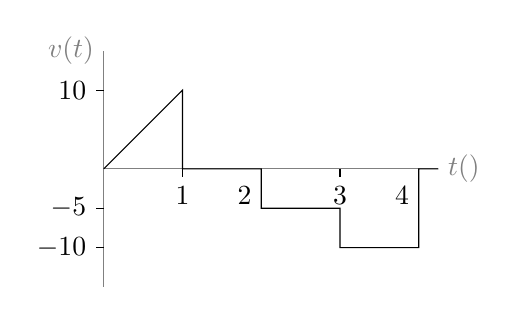
\begin{tikzpicture}
\draw[gray](0,0)--(4.25,0)node[right]{$t(\si{\milli\second})$};
\draw[gray](0,-1.5)--(0,1.5)node[left]{$v(t)$};
\draw(0,0)--(1,1)--(1,0)--(2,0)--(2,-0.5)--(3,-0.5)--(3,-1)--(4,-1)--(4,0)--(4.25,0);
\draw(0,1)--++(-0.1,0)node[left]{$\SI{10}{\volt}$};
\draw(0,-1)--++(-0.1,0)node[left]{$\SI{-10}{\volt}$};
\draw(0,-0.5)--++(-0.1,0)node[left]{$\SI{-5}{\volt}$};
\draw(1,0)--++(0,-0.1)node[below]{$1$};
\draw(2,0)--++(0,-0.1)node[below left]{$2$};
\draw(3,0)--++(0,-0.1)node[below]{$3$};
\draw(4,0)--++(0,-0.1)node[below left]{$4$};
\end{tikzpicture}
\caption*{(الف)}
\end{subfigure}%
\begin{subfigure}{0.5\textwidth}
\centering
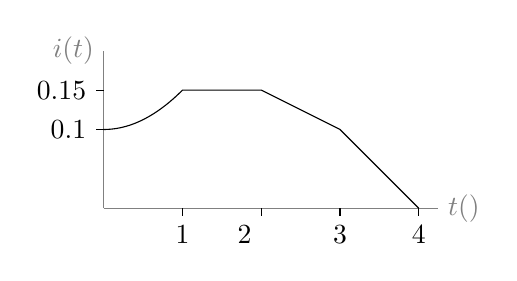
\begin{tikzpicture}
\draw[gray](0,0)--(4.25,0)node[right]{$t(\si{\milli\second})$};
\draw[gray](0,0)--(0,2)node[left]{$i(t)$};
\draw(0,1)
\foreach \kx in {0,0.01,...,1}{--(\kx,1+0.5*\kx*\kx)}--(1,1.5)--(2,1.5)--(3,1)--(4,0);
\draw(0,1)--++(-0.1,0)node[left]{$\SI{0.1}{\ampere}$};
\draw(0,1.5)--++(-0.1,0)node[left]{$\SI{0.15}{\ampere}$};
%\draw(0,-0.5)--++(-0.1,0)node[left]{$\SI{-5}{\volt}$};
\draw(1,0)--++(0,-0.1)node[below]{$1$};
\draw(2,0)--++(0,-0.1)node[below left]{$2$};
\draw(3,0)--++(0,-0.1)node[below]{$3$};
\draw(4,0)--++(0,-0.1)node[below]{$4$};
\end{tikzpicture}
\caption*{(ب)}
\end{subfigure}%
\caption{مشق \حوالہ{مشق_امالہ_رو_دباو_خط_پ} کا دور۔}
\label{شکل_امالہ_مشق_رو_دباو_خط_پ}
\end{figure}

جواب:رو کا خط شکل \حوالہ{شکل_امالہ_مشق_رو_دباو_خط_پ} میں دکھایا گیا ہے۔لمحہ \عددی{t=\SI{3}{\milli\second}} پر \عددی{w_L(\SI{3}{\milli\second})=\SI{0.5}{\milli\joule}} ہے۔
\انتہا{مشق}
%=============================
\ابتدا{مشق}\شناخت{مشق_امالہ_رو_دباو_خط_ت}
شکل \حوالہ{شکل_امالہ_مشق_رو_دباو_خط_ت} میں \عددی{\SI{1}{\milli\henry}}، \عددی{\SI{4}{\milli\henry}}، \عددی{\SI{3}{\micro\farad}} اور \عددیء{\SI{4}{\micro\farad}} میں ذخیرہ توانائی دریافت کریں۔

\begin{figure}
\centering
\begin{tikzpicture}
\draw(0,0) to [american voltage source,l={$\SI{10}{\volt}$}]++(0,\y) to [resistor,l={$\SI{2}{\ohm}$}]++(0,\y) to [short]++(\x,0) to [inductor,l={$\SI{1}{\milli\henry}$}]++(\x,0) to [resistor,l={$\SI{6}{\ohm}$}]++(\x,0) to [inductor,l={$\SI{4}{\milli\henry}$}]++(\x,0) to [resistor,l={$\SI{10}{\ohm}$}]++(0,-2*\y) to [short] (0,0);
\draw(\x,2*\y) to [short,*-]++(0,\y) to [american current source,l={$\SI{2}{\ampere}$}]++(3*\x,0) to [short,-*]++(0,-\y);
\draw(\x,0) to [capacitor,*-*,l={$\SI{3}{\micro\farad}$}]++(0,2*\y);
\draw(2*\x,0) to [resistor,*-,l={$\SI{8}{\ohm}$}]++(0,\y) to [capacitor,-*,l={$\SI{4}{\micro\farad}$}]++(0,\y);
\end{tikzpicture}
\caption{مشق \حوالہ{مشق_امالہ_رو_دباو_خط_ت} کا دور۔}
\label{شکل_امالہ_مشق_رو_دباو_خط_ت}
\end{figure}

جوابات:\عددی{\SI{302}{\micro\joule}}، \عددی{\SI{0.907}{\micro\joule}}، \عددی{\SI{85.6}{\micro\joule}}، \عددی{\SI{114}{\micro\joule}}
\انتہا{مشق}
%=============================

\حصہ{برق گیر اور امالہ گیر کے خصوصیات}
برقی گنجائش، برقی گنجائش  کی قیمت میں خلل اور دباو، برق گیر کے  اہم خصوصیات ہیں۔ معیاری برق گیر چند \عددی{\si{\pico\farad}} سے تقریباً \عددی{\SI{50}{\milli\farad}} تک کی قیمتوں میں عام دستیاب ہے۔ان سے کم اور زیادہ قیمتیں بھی دستیاب ہیں۔ یہ برق گیر عموماً \عددی{\SI{6.3}{\volt}} تا \عددی{\SI{500}{\volt}} تک کے مختلف دباو کے لئے دستیاب ہیں۔زیادہ دباو کے برق گیر بھی دستیاب ہیں۔برق گیر کو اس کی معین دباو سے زیادہ دباو پر ہرگز استعمال نہ کریں چونکہ ایسا کرنے سے  برق گیر تباہ ہو سکتا ہے۔برقی گنجائش میں خلل کی عمومی قیمتیں \عددی{\SI{\mp 5}{\percent}}، \عددی{\SI{\mp 10}{\percent}} اور \عددی{\SI{\mp 20}{\percent}} ہیں۔ جدول \حوالہ{جدول_امالہ_معیاری_برقی_گنجائش} میں معیاری دستیاب برقی گیر کی گنجائش دی گئی ہے۔
%==============================

\begin{table}\caption{معیاری برق گیر کے گنجائش کی قیمتیں۔}
\centering
\begin{tabular}{lllllllllll}
$\si{\pico\farad}$ & $\si{\pico\farad}$ & $\si{\pico\farad}$ & $\si{\pico\farad}$ & $\si{\micro\farad}$ & $\si{\micro\farad}$ &  $\si{\micro\farad}$ &  $\si{\micro\farad}$ &  $\si{\micro\farad}$ &  $\si{\micro\farad}$ &  $\si{\micro\farad}$ \\
\hline
$1$ & $10$ &$100$ & $1000$ &$0.010$ & $0.10$ &$1.0$ & $10$ &$100$ & $1000$ & $\num{10000}$\\
 & $12$ &$120$ & $1200$ &$0.012$ & $0.12$ &$1.2$ & $12$ &$120$ & $1200$ & $\num{12000}$\\
 $1.5$& $15$ &$150$ & $1500$ &$0.015$ & $0.15$ &$1.5$ & $15$ &$150$ & $1500$ & $\num{15000}$\\
 & $18$ &$180$ & $1800$ &$0.018$ & $0.18$ &$1.8$ & $18$ &$180$ & $1800$ & $\num{18000}$\\
$2$ & $20$ &$200$ & $2000$ &$0.020$ & $0.20$ &$2.0$ & $20$ &$200$ & $2000$ & $\num{20000}$\\
 & $22$ &$220$ & $2200$ &$0.022$ & $0.22$ &$2.2$ & $22$ &$220$ & $2200$ & $\num{22000}$\\
 & $27$ &$270$ & $2700$ &$0.027$ & $0.27$ &$2.7$ & $27$ &$270$ & $2700$ & $\num{27000}$\\
$3$ & $33$ &$330$ & $3300$ &$0.330$ & $0.33$ &$3.3$ & $33$ &$330$ & $3300$ & $\num{33000}$\\
$4$ & $39$ &$390$ & $3900$ &$0.390$ & $0.39$ &$3.9$ & $39$ &$390$ & $3900$ & $\num{39000}$\\
$5$ & $47$ &$470$ & $4700$ &$0.470$ & $0.47$ &$3.3$ & $47$ &$470$ & $4700$ & $\num{47000}$\\
$6$ & $51$ &$510$ & $5100$ &$0.510$ & $0.51$ &$3.3$ & $51$ &$510$ & $5100$ & $\num{51000}$\\
$7$ & $56$ &$560$ & $5600$ &$0.560$ & $0.56$ &$3.3$ & $56$ &$560$ & $5600$ & $\num{56000}$\\
$8$ & $68$ &$680$ & $6800$ &$0.680$ & $0.68$ &$3.3$ & $68$ &$680$ & $6800$ & $\num{68000}$\\
$9$ & $82$ &$820$ & $8200$ &$0.820$ & $0.82$ &$3.3$ & $82$ &$820$ & $8200$ & $\num{82000}$
\end{tabular}
\label{جدول_امالہ_معیاری_برقی_گنجائش}
\end{table}
%==============================

امالہ گیر کو موصل تار سے بنایا جاتا ہے لہٰذا نہ چاہتے ہوئے بھی اس کی مزاحمت ہو گی۔ امالہ گیر کے اہم خصوصیات اس کی امالہ اور مزاحمت ہیں۔امالہ گیر \عددی{\SI{1}{\nano\henry}} تا \عددی{\SI{100}{\milli\henry}} کی قیمتوں میں عام دستیاب ہے۔اس سے کم یا زیادہ قیمتیں بھی دستیاب ہیں۔امالہ کی قیمتیں \عددی{\SI{\mp 5}{\percent}} اور \عددی{\SI{\mp 10}{\percent}} کے خلل میں دستیاب ہیں۔جدول \حوالہ{جدول_امالہ_امالہ_عمومی_دستیاب_قیمتیں} میں امالہ کی عمومی دستیاب قیمتیں دی گئی ہیں۔

\begin{table}\caption{امالہ کی عمومی دستیاب قیمتیں۔}
\centering
\begin{tabular}{lllllllll}
$\si{\nano\henry}$ & $\si{\nano\henry}$ &$\si{\nano\henry}$ &$\si{\micro\henry}$ &$\si{\micro\henry}$ &$\si{\micro\henry}$ &$\si{\milli\henry}$ &$\si{\milli\henry}$ &$\si{\milli\henry}$ \\
\hline
$1$ & $10$ &$100$ & $1.0$ & $10$ &$100$ & $1.0$ & $10$ & $100$ \\
$1.2$ & $12$ &$120$ & $1.2$ & $12$ &$120$ & $1.2$ & $12$ &  \\
$1.5$ & $15$ &$150$ & $1.5$ & $15$ &$150$ & $1.5$ & $15$ &  \\
$1.8$ & $18$ &$180$ & $1.8$ & $18$ &$180$ & $1.8$ & $18$ &  \\
$2$ & $20$ &$200$ & $2.0$ & $20$ &$200$ & $2.0$ & $20$ &  \\
$2.2$ & $22$ &$220$ & $2.2$ & $22$ &$220$ & $2.2$ & $22$ &  \\
$2.7$ & $27$ &$270$ & $2.7$ & $27$ &$270$ & $2.7$ & $27$ &  \\
$3$ & $33$ &$330$ & $3.3$ & $33$ &$330$ & $3.3$ & $33$ &  \\
$4$ & $39$ &$390$ & $3.9$ & $39$ &$390$ & $3.9$ & $39$ &  \\
$5$ & $47$ &$470$ & $4.7$ & $47$ &$470$ & $4.7$ & $47$ &  \\
$6$ & $51$ &$510$ & $5.1$ & $51$ &$510$ & $5.1$ & $51$ &  \\
$7$ & $56$ &$560$ & $5.6$ & $56$ &$560$ & $5.6$ & $56$ &  \\
$8$ & $68$ &$680$ & $6.8$ & $68$ &$680$ & $6.8$ & $68$ &  \\
$9$ & $82$ &$820$ & $8.2$ & $82$ &$820$ & $8.2$ & $82$ &  
\end{tabular}
\label{جدول_امالہ_امالہ_عمومی_دستیاب_قیمتیں}
\end{table}

%===================
\ابتدا{مثال}\شناخت{مثال_امالہ_گنجائش_اور_قیمتیں_الف}
شکل \حوالہ{شکل_امالہ_گنجائش_اور_قیمتیں_الف}-الف میں \عددی{\SI{100}{\nano\farad}} برق گیر کا دباو دکھایا گیا ہے۔برقی گنجائش میں خلل \عددی{\SI{\mp 10}{\percent}} ممکن ہے۔کم سے کم اور زیادہ سے زیادہ گنجائش کی صورت میں رو کے خط حاصل کریں۔اس برقی گنجائش کو عموماً \عددی{\SI{100}{\nano\farad}\SI{\mp10}{\percent}} لکھا جاتا ہے۔

\begin{figure}
\centering
\begin{subfigure}{0.5\textwidth}
\centering
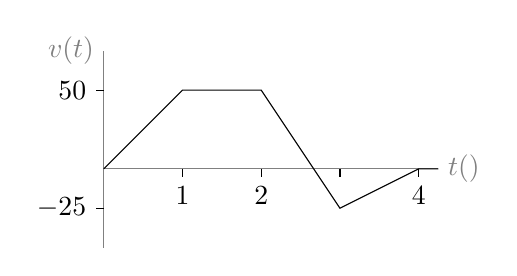
\begin{tikzpicture}
\draw[gray](0,-1)--(0,1.5)node[left]{$v(t)$};
\draw[gray](0,0)--(4.25,0)node[right]{$t(\si{\micro\second})$};
\draw(0,0)--(1,1)--(2,1)--(3,-0.5)--(4,0)--(4.25,0);
\draw(0,1)--++(-0.1,0)node[left]{$\SI{50}{\volt}$};
\draw(0,-0.5)--++(-0.1,0)node[left]{$\SI{-25}{\volt}$};
\draw(1,0)--++(0,-0.1)node[below]{$1$};
\draw(2,0)--++(0,-0.1)node[below]{$2$};
\draw(3,0)--++(0,-0.1);
\draw(4,0)--++(0,-0.1)node[below]{$4$};
\end{tikzpicture}
\caption*{(الف) برق گیر کا دباو۔}
\end{subfigure}%
\begin{subfigure}{0.5\textwidth}
\centering
\begin{tikzpicture}
\draw[gray](0,-1.75)--(0,1.5)node[left]{$i(t)$};
\draw[gray](0,0)--(4.25,0)node[right]{$t(\si{\micro\second})$};
\draw(0,0)--(0,1)--(1,1)--(1,0)--(2,0)--(2,-1.5)--(3,-1.5)--(3,0.5)--(4,0.5)--(4,0)--(4.25,0);
\draw(0,1)--++(-0.1,0)node[left]{$\SI{5.5}{\ampere}$};
\draw(0,0.5)--++(-0.1,0)node[left]{$\SI{2.75}{\ampere}$};
\draw(0,-1.5)--++(-0.1,0)node[left]{$\SI{-8.25}{\ampere}$};
\draw(1,0)node[below]{$1$};
\draw(2,0)node[below left]{$2$};
\draw(3,0)node[below right]{$3$};
\draw(4,0)node[below]{$4$};
\end{tikzpicture}
\caption*{(ب) \عددی{\SI{110}{\nano\farad}} کی رو۔}
\end{subfigure}
\begin{subfigure}{0.5\textwidth}
\centering
\begin{tikzpicture}
\draw[gray](0,-1.75)--(0,1.5)node[left]{$i(t)$};
\draw[gray](0,0)--(4.25,0)node[right]{$t(\si{\micro\second})$};
\draw(0,0)--(0,0.818)--(1,0.818)--(1,0)--(2,0)--(2,-1.23)--(3,-1.23)--(3,0.41)--(4,0.41)--(4,0)--(4.25,0);
\draw(0,0.818)--++(-0.1,0)node[left]{$\SI{4.5}{\ampere}$};
\draw(0,0.41)--++(-0.1,0)node[left]{$\SI{2.25}{\ampere}$};
\draw(0,-1.23)--++(-0.1,0)node[left]{$\SI{-6.75}{\ampere}$};
\draw(1,0)node[below]{$1$};
\draw(2,0)node[below left]{$2$};
\draw(3,0)node[below right]{$3$};
\draw(4,0)node[below]{$4$};
\end{tikzpicture}
\caption*{(پ) \عددی{\SI{90}{\nano\farad}} کی رو۔}
\end{subfigure}%
\caption{مثال \حوالہ{مثال_امالہ_گنجائش_اور_قیمتیں_الف} کا دور۔}
\label{شکل_امالہ_گنجائش_اور_قیمتیں_الف}
\end{figure}

حل:برق گیر کی زیادہ سے زیادہ قیمت دی گئی قیمت سے \عددی{\SI{10}{\percent}} زیادہ ہو سکتی ہے۔یوں اس کی زیادہ سے زیادہ گنجائش \عددی{\SI{110}{\nano\farad}} ممکن ہے۔اس قیمت کے گنجائش کی رو کو شکل \حوالہ{شکل_امالہ_گنجائش_اور_قیمتیں_الف}-ب میں دکھایا گیا ہے جہاں پہلے ایک مائیکرو سیکنڈ میں دباو کی تبدیلی کی شرح 
\begin{align*}
\frac{\dif v}{\dif t}=\frac{50-0}{\SI{1}{\micro\second}-\SI{0}{\micro\second}}=\SI{50}{\mega \volt \per\second}
\end{align*} 
ہونے کی بنا اس دورانیے کی رو
\begin{align*}
i=C \frac{\dif v}{\dif t}=110 \times 10^{-9} \times 50 \times 10^{6}=\SI{5.5}{\ampere}
\end{align*}
ہے۔اگلے ایک مائیکرو سیکنڈ میں دباو تبدیل نہیں ہوتا لہٰذا \عددی{\frac{\dif v}{\dif t}=0} ہے اور یوں رو بھی صفر کے برابر ہے۔دورانیہ \عددی{t=\SI{2}{\micro\second}} تا  \عددی{t=\SI{3}{\micro\second}} دباو کی شرح تبدیلی
\begin{align*}
\frac{\dif v}{\dif t}=\frac{-25-50}{\SI{3}{\micro\second}-\SI{2}{\micro\second}-\SI{0}{\micro\second}}=\SI{-75}{\mega \volt \per\second}
\end{align*}
ہے لہٰذا رو
\begin{align*}
i=C \frac{\dif v}{\dif t}=110 \times 10^{-9} \times \left(-75 \times 10^{6}\right)=\SI{-8.25}{\ampere}
\end{align*}
ہو گی۔دورانیہ \عددی{t=\SI{3}{\micro\second}} تا  \عددی{t=\SI{4}{\micro\second}} دباو کی شرح تبدیلی
\begin{align*}
\frac{\dif v}{\dif t}=\frac{0-(-25)}{\SI{4}{\micro\second}-\SI{3}{\micro\second}-\SI{0}{\micro\second}}=\SI{25}{\mega \volt \per\second}
\end{align*}
ہے لہٰذا رو
\begin{align*}
i=C \frac{\dif v}{\dif t}=110 \times 10^{-9} \times 25\times 10^{6}=\SI{2.75}{\ampere}
\end{align*}
ہو گی۔

خلل کی قیمت سے برق گیر کی کم سے کم ممکنہ گنجائش \عددی{\SI{90}{\nano\farad}} حاصل ہوتی ہے۔دباو کی تبدیلی کی شرح استعمال کرتے ہوئے رو درج ذیل حاصل ہوتی ہے۔
\begin{equation*}
i=
\begin{cases}
90 \times 10^{-9} \times 50 \times 10^{6}=\SI{4.5}{\ampere} & \SI{0}{\micro\second} \le t \le \SI{1}{\micro\second}\\
90 \times 10^{-9} \times 0=\SI{0}{\ampere} & \SI{1}{\micro\second} \le t \le \SI{2}{\micro\second}\\
90 \times 10^{-9} \times (-75) \times 10^{6}=\SI{-6.75}{\ampere} & \SI{2}{\micro\second}  \le t \le \SI{3}{\micro\second}\\
90 \times 10^{-9} \times 25 \times 10^{6}=\SI{2.25}{\ampere} & \SI{3}{\micro\second}  \le t \le \SI{4}{\micro\second}
\end{cases}
\end{equation*}
\انتہا{مثال}
%======================

\حصہ{سلسلہ وار جڑے برق گیر}
شکل \حوالہ{شکل_امالہ_متعدد_سلسلہ_وار_برق_گیر_مساوی_حصول} میں متعدد برق گیر سلسلہ وار جڑے دکھائے گئے ہیں۔تمام سلسلہ وار جڑے پرزوں میں رو کی قیمت یکساں ہوتی ہے۔کرخوف قانون دباو سے اس دور کے لئے درج ذیل لکھا جا سکتا ہے۔
\begin{align*}
v(t)=v_1(t)+v_2(t)+v_3(t)+\cdots +v_N(t)
\end{align*}
انفرادی برق گیر کے لئے
\begin{align*}
q(t)&=C_1 v_1(t)\\
q(t)&=C_2 v_2(t)\\
q(t)&=C_3 v_3(t)\\
& \vdots\\
q(t)&=C_N v_N(t)\\
\end{align*}
لکھا جا سکتا ہے جہاں \عددی{t} دورانیے میں رو \عددی{i(t)} ہر برق گیر پر برابر \عددی{q(t)} کا بار جمع کرتی ہے۔ مندرجہ بالا دو مساوات کو ملاتے ہوئے
\begin{align*}
v(t)&=\frac{q(t)}{C_1}+\frac{q(t)}{C_2}+\frac{q(t)}{C_3}+\cdots +\frac{q(t)}{C_N}\\
&=q(t)\left(\frac{1}{C_1}+\frac{1}{C_2}+\frac{1}{C_3}+\cdots+\frac{1}{C_N}\right)
\end{align*}
لکھا جا سکتا ہے۔اس مساوات میں
\begin{align}\label{مساوات_امالہ_سلسلہ_وار_برق_گیر_کا_مساوی}
\frac{1}{C_S}=\frac{1}{C_1}+\frac{1}{C_2}+\frac{1}{C_3}+\cdots+\frac{1}{C_N}
\end{align}
لکھتے ہوئے اسے
\begin{align*}
v(t)=\frac{q(t)}{C_S}
\end{align*}
یعنی
\begin{align}
q(t)=C_S v(t)
\end{align}
 صورت میں لکھا جا سکتا ہے جو ایک عدد برقی گیر کی مساوات ہے۔مساوات \حوالہ{مساوات_امالہ_سلسلہ_وار_برق_گیر_کا_مساوی} متعدد سلسلہ وار جڑے برق گیروں کا مساوی برق گیر دیتی ہے۔

\begin{figure}
\centering
\begin{subfigure}{1\textwidth}
\centering
\begin{tikzpicture}
\draw(0,0) to [short,i={$i(t)$},o-]++(\x/2,0) to [capacitor,l={$C_1$}]++(\x,0) to [capacitor,l={$C_2$}]++(\x,0) to [capacitor,l={$C_3$}]++(\x,0)coordinate(kup);
\draw[dashed](kup)--++(\x/4,0)--++(0,-\y)--++(-2*\x-\x/2,0)coordinate(klow);
\draw(klow) to [capacitor,l_={$C_N$}]++(-\x,0) to [short,-o]++(-\x/4,0);
\draw(0,-\y/2)node{$\begin{aligned} &+ \\ &v(t)\\ &- \end{aligned}$};
\draw(\x/2+\x/2,-2*\dy)node[below]{$+ \, v_1(t) \, -$};
\draw(\x/2+\x/2+\x,-2*\dy)node[below]{$+ \, v_2(t) \, -$};
\draw(\x/2+\x/2+2*\x,-2*\dy)node[below]{$+ \, v_3(t) \, -$};
\draw(\x/4+\x/2,-\y-2*\dy)node[below]{$- \, v_N(t) \, +$};
\end{tikzpicture}
\caption*{(الف) متعدد سلسلہ وار جڑے برق گیر۔}
\end{subfigure}
\begin{subfigure}{1\textwidth}
\centering
\begin{tikzpicture}
\draw(0,0) to [short,i={$i(t)$},o-]++(\x,0) to [capacitor,l={$C_S$}]++(0,-\y) to [short,-o]++(-\x,0);
\draw(0,-\y/2)node{$\begin{aligned} &+ \\ &v(t)\\ &- \end{aligned}$};
\end{tikzpicture}
\caption*{(ب) متعدد سلسلہ وار جڑے برقی گیروں کا مساوی برق گیر۔}
\end{subfigure}
\caption{متعدد سلسلہ وار جڑے برق گیر کے مساوی برق گیر کا حصول۔}
\label{شکل_امالہ_متعدد_سلسلہ_وار_برق_گیر_مساوی_حصول}
\end{figure}
